\section{Durchführung}
\label{sec:Durchführung}
Der Versuch ist wie in Abbildung \ref{pic:aufbau} aufgebaut. 
Als Lichtquelle dient eine Halogen-Lampe ($\SI{12}{\volt}$; $\SI{50}{\watt}$).
Mit Hilfe von Interferenzfiltern kann die Strahlung monochromatisiert werden.
Es liegen 9 Interferenzfilter von $\SI{1.06}{\micro\meter}$ bis $\SI{2.65}{\micro\meter}$ vor.
\begin{figure}
    \centering
    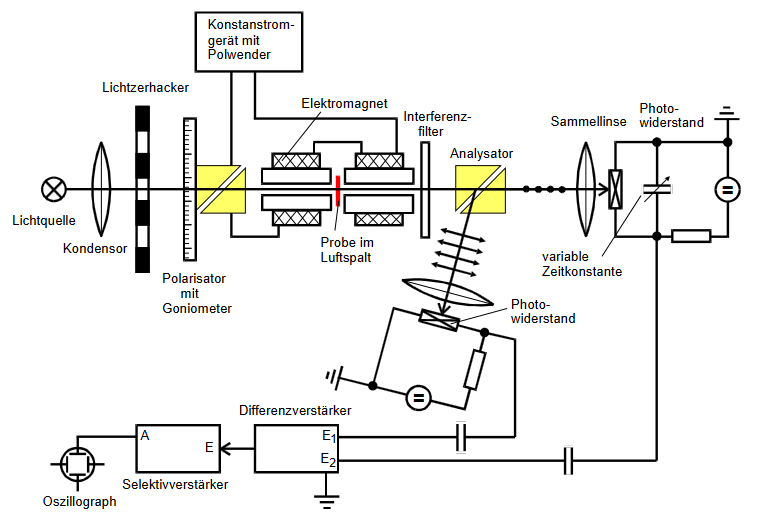
\includegraphics[width = 0.78\textwidth]{pics/aufbau.png}
    \caption{Unterscheidung nach Bandlücke.\cite{Anleitung}}
    \label{pic:aufbau}
\end{figure}
Mit Hilfe eines Glan-Thompson Prismas aus Kalkspat wird das Licht linear-polarisiert. In einem großen Elektromagnet wird in einem Luftspalt die Probe eingeführt.
Für ein zeitlich konstantes Magnetfeld wird die Wicklung des Magneten mit einem Konstantstromgerät gespeist.
Ein doppelter Drehwinkel kann mit einer Umpolung des Feldes erreicht werden.
Die Lichtintensität wird mit Photowiderständen aus PbS gemessen. 
Vor den Photowiderständen wird ein weiteres Glan-Thompson Prisma plaziert, sodass der Strahl in zwei um $\ang{90}$ rotierte linear polarisierte Strahlen aufgeteilt wird.
Durch einen Differenzverstärker werden die Lichtintensitäten von den beiden Photowiderständen subtrahiert und verstärkt.
Um Rauschspannungen an den Photowiderständen zu reduzieren, wird der Strahl mit einem Lichtzerhacker
gepulst und am Ende an einen Selektivverstärker auf die Zerhackerfrequenz eingestellt.
Das Ausgangssignal des Selektivverstärkers wird an ein Oszilloskop angeschlossen.
Bei einer minimalen Differenzspannung ist die Polarisationsebene bei einem Winkel von $\ang{45}$. 

\subsection{Justierung und Messung}
Der erste Teil der Justage prüft die Arbeitsweise der Polarisationsvorrichtung. 
Dazu wird geschaut, ob bei einer Drehung des Polarisators die Lichtintensität des durchgehenden Strahls bei geeigneter Stellung verschwindet. 
Ist dies nicht der Fall, wird das Analysatorprisma vorsichtig um seine vertikale Achse gedreht bis die Lichtintensität verschwindet.

Im nächsten Schritt werden die Lichtschutzhauben zwischen Sammellinse und Photowiderstand entfernt. 
Durch Rotation des Polarisators sollte das Licht zwischen den Photowiderständen hin und her geschaltet werden können.

Zuletzt wird der Selektivverstärker auf die Lichtzerhackerfrequenz eingestellt. Dafür wird einer der Photowiderstände an den Selektivverstärker angeschlossen und mit Hilfe der
Frequenzstellknöpfe auf den maximalen Wert eingestellt. Dabei wird eine Zerhackerfrequenz von etwa $f = \SI{450}{\Hz}$ eingestellt.
Der Gütefaktor wird für die Messung auf $Q = 100$ gestellt.
\\
Zuerst wird nach der Justage die Kraftflussdichte $B(z)$ in Richtung des einfallenden Lichtes in der nähe des Luftspaltes mit einer Hallsonde vermessen.
Daraufhin wird die Faraday-Rotation an einer hochreinen GaAs-Probe ($d = \SI{5.11}{\milli\meter}$)
und zwei n-dotierten GaAs-Proben mit $N = \SI{1.2e18}{\cm^{-3}}$ beziehungsweise $d = \SI{1.36}{\milli\meter}$ (Probe 1) und $N = \SI{2.8e18}{\cm^{-3}}$ beziehungsweise $d = \SI{1.296}{\milli\meter}$ (Probe 2) gemessen.
Dabei wird für jede Probe die Faraday-Rotation jeweils mit den neun Interfenzfiltern und beiden Magnetfeldpolungen vermessen.